%%%%%%%%%%%%%%%%%%%%%%%%%%%%%%%%%%%%%%%%%
% Journal Article
% LaTeX Template
% Version 1.4 (15/5/16)
%
% This template has been downloaded from:
% http://www.LaTeXTemplates.com
%
% Original author:
% Frits Wenneker (http://www.howtotex.com) with extensive modifications by
% Vel (vel@LaTeXTemplates.com)
%
% License:
% CC BY-NC-SA 3.0 (http://creativecommons.org/licenses/by-nc-sa/3.0/)
%
%%%%%%%%%%%%%%%%%%%%%%%%%%%%%%%%%%%%%%%%%

%----------------------------------------------------------------------------------------
%	PACKAGES AND OTHER DOCUMENT CONFIGURATIONS
%----------------------------------------------------------------------------------------

\documentclass[twoside,twocolumn]{article}

\usepackage{blindtext} % Package to generate dummy text throughout this template 

\usepackage[sc]{mathpazo} % Use the Palatino font
\usepackage[T1]{fontenc} % Use 8-bit encoding that has 256 glyphs
\linespread{1.05} % Line spacing - Palatino needs more space between lines
\usepackage{microtype} % Slightly tweak font spacing for aesthetics

\usepackage[dutch]{babel} % Language hyphenation and typographical rules

\usepackage[hmarginratio=1:1,top=32mm,columnsep=20pt]{geometry} % Document margins
\usepackage[hang, small,labelfont=bf,up,textfont=it,up]{caption} % Custom captions under/above floats in tables or figures
\usepackage{booktabs} % Horizontal rules in tables

\usepackage{lettrine} % The lettrine is the first enlarged letter at the beginning of the text

\usepackage{enumitem} % Customized lists
\setlist[itemize]{noitemsep} % Make itemize lists more compact

\usepackage{abstract} % Allows abstract customization
\renewcommand{\abstractnamefont}{\normalfont\bfseries} % Set the "Abstract" text to bold
\renewcommand{\abstracttextfont}{\normalfont\small\itshape} % Set the abstract itself to small italic text

\usepackage{titlesec} % Allows customization of titles
\renewcommand\thesection{\Roman{section}} % Roman numerals for the sections
\renewcommand\thesubsection{\roman{subsection}} % roman numerals for subsections
\titleformat{\section}[block]{\large\scshape\centering}{\thesection.}{1em}{} % Change the look of the section titles
\titleformat{\subsection}[block]{\large}{\thesubsection.}{1em}{} % Change the look of the section titles

\usepackage{fancyhdr} % Headers and footers
\pagestyle{fancy} % All pages have headers and footers
\fancyhead{} % Blank out the default header
\fancyfoot{} % Blank out the default footer
\fancyhead[C]{} % Custom header text
\fancyfoot[RO,LE]{\thepage} % Custom footer text

\usepackage{titling} % Customizing the title section

\usepackage{hyperref} % For hyperlinks in the PDF
\usepackage{graphicx}

%----------------------------------------------------------------------------------------
%	TITLE SECTION
%----------------------------------------------------------------------------------------

\setlength{\droptitle}{-4\baselineskip} % Move the title up

\pretitle{\begin{center}\Huge\bfseries} % Article title formatting
\posttitle{\end{center}} % Article title closing formatting
\title{Grote gegevens en denderende data: hoe slaan websites hun data op?} % Article title
\author{%
\textsc{Florian Dejonckheere} \\[1ex] % Your name
\normalsize Hogeschool Gent \\ % Your institution
\normalsize \href{mailto:florian@dejonckhee.re}{florian@dejonckhee.re} % Your email address
%\and % Uncomment if 2 authors are required, duplicate these 4 lines if more
%\textsc{Jane Smith}\thanks{Corresponding author} \\[1ex] % Second author's name
%\normalsize University of Utah \\ % Second author's institution
%\normalsize \href{mailto:jane@smith.com}{jane@smith.com} % Second author's email address
}
\date{\today} % Leave empty to omit a date

%----------------------------------------------------------------------------------------

\begin{document}

% Print the title
\maketitle

%----------------------------------------------------------------------------------------
%	ARTICLE CONTENTS
%----------------------------------------------------------------------------------------

%% Introduction

\textbf{De laatste jaren zijn grootschalige sociale mediaplatformen zoals Twitten en Facebook sterk opgekomen.
  Door het toenemende gebruik ervan is de digitale voetafdruk van de gemiddelde internetgebruiker ook massief gestegen.
  Deze websites hebben dan ook te maken met een zondvloed van gegevens die opgeslagen moeten worden, klaar om ze snel naar de gebruiker te sturen.
  Maar hoe worden die gegevens precies opgeslagen? We bekijken het voorbeeld van Open Webslides.}\\

%% Body
\section*{Open Webslides}

Open Webslides is een online collaboratieplatform voor leerkrachten en leerlingen.
Hierbij wordt er door beide partijen aan dezelfde cursus gesleuteld, zodat studenten deze beter kunnen leren en leerkrachten gemakkelijk feedback kunnen verwerken.

Het deel van Open Webslides waar we ge\"{i}nteresseerd in zijn, is de feed van de \textit{recente activiteit}.
Deze feed ziet er een beetje uit zoals de feed op Facebook of Twitter.
De meest recentste berichten staan bovenaan, de minder recentere berichten gaan eronder.
Natuurlijk gaat het hier niet over foto's en evenementen, maar wel over wie iets veranderd heeft op de cursus, en wat precies.
Zo kan je in \'{e}\'{e}n oogopslag zien wanneer de leerkracht een hoofdstuk heeft toegevoegd, of dat een van je medestudenten een vraag heeft gesteld bij een onduidelijke zin.


\begin{figure}
  \centering
  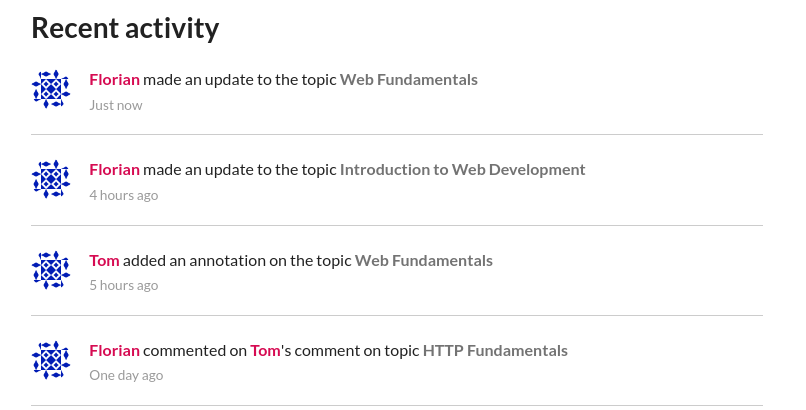
\includegraphics[width=.8\textwidth]{recent-activity.png}
  \caption{Recent activiteits-feed}
  \label{fig:graph-model}
\end{figure}

Maar hoe slaan we deze gegevens precies op?
Bij elk item hoort een cursus, een auteur en de actie die uitgevoerd werd.
En natuurlijk ook het tijdstip van de actie, waarop we ook moeten sorteren vooraleer de lijst naar de gebruiker te sturen.

\section*{Databanken}

Er kan gekozen worden uit de vele, al bestaande databanktoepassingen.
Maar eerst moeten we kiezen welk type databank het best past: een \textit{relationele}, een \textit{document}- of een \textit{graafdatabank}.
Bij een relationele databank worden de gegevens opgeslaan in tabellen: elke tabel heeft kolommen, en elk item heeft een waarde voor deze kolommen.
Dit is de traditionele manier van gegevens opslaan.
Het laat ons toe om gemakkelijk te zoeken in alle gegevens, en deze te sorteren.
Dat komt goed van pas als we alle items willen sorteren op tijdstip.
Het combineren van gegevens in verschillende tabellen -- bijvoorbeeld een tabel voor auteur, en een andere tabel voor cursussen -- gaat zeer snel in een relationele databank.

Een document-databank daarentegen, slaat alle gegevens op als een document: een ondoorzichtig stuk data waar er niet in gezocht kan worden.
Om dit te omzeilen, steken we alle gegevens die nodig zijn in eenzelfde document.
In ons geval wil dit dus zeggen dat de auteur, cursus en acties in hetzelfde document zitten.
Document-databanken zijn typisch zeer goed in het afhandelen van massieve datastromen. 
Dat kan in ons voordeel spelen als we een systeem overwegen met duizenden gebruikers.

Ten laatste kunnen we ook kiezen voor een graafdatabank.
Een graaf is een verzameling van punten of objecten, en die verbonden zijn door lijnen.
Het doorkruisen van lijnen van object tot object is een zeer snelle actie.
Dat komt goed uit voor de gelinkte datastructuur van Open Webslides.

%% Results


Aangezien relationele databanken niet de focus zijn van het onderzoek, moet er uiteindelijk gekozen worden tussen een document- en een graafdatabank.
Hiervoor gaan we een schema opstellen, en dat in elke databank invoegen.
We doornemen ook een aantal realistische scenarios om deze databank te gebruiken.
Aan de hand van deze twee elementen kunnen we testen welke databank het beste ophoudt aan de (gesimuleerde) stress van duizenden gebruikers.
Het verdict: de graafdatabank is 10 tot in bepaalde gevallen zelfs 40 keer trager dan de document-databank.
Een duidelijke overwinning dus!

%% Conclusion

\section*{Conlusie}

Het is dus duidelijk voor het Open Webslides project: document-databanken bieden dus de meest effici\"{e}nte oplossing.

We hebben nu een kijkje genomen achter de schermen in de wereld van data-opslag op grote schaal.
We zagen hoe bedrijven zoals Facebook en Twitter de massieve vloed aan data opslaan.
Het verschil tussen de databanktoepassingen is nu ook duidelijk: relationele, document- en graafdatabanken.

Mensen staan zelden stil bij de technologie die achter social media websites zitten, en welke hordes de ontwikkelaar heeft moeten nemen om deze technologie\"{e}n naar een groot publiek te brengen.
Denk daar maar eens over na, bij de volgende gedachteloze scroll van je Facebook feed!

\end{document}
